{ %section6_1
	\subsection{Порядок выполнения работы}
	\Large
	\begin{enumerate}
		\itemЗаменить функцию rand на rand\textunderscore r и объяснить в отчёте, чем эти функции различаются, а также привести условия, при которых использование rand вместо rand\textunderscore r приведёт к ошибочным результатам работы. 
		\itemИспользуя функцию omp\textunderscore get\textunderscore wtime, измерить время выполнения каждого из пяти этапов программы (заполнение массива, умножение матриц и т.п.). Замер времени необходимо осуществить двумя методами:	
			\begin{itemize}
				\itemметод А – как среднее по 100 прогонам (использовать srand(i));
				\itemметод Б – как минимальное по 100 прогонам (использовать srand(константа)).	
			\end{itemize}
		\itemВывод в консоль (или в файл) информации о замеренном времени выполнения этапов нужно вынести за пределы основного цикла for (чтобы при распараллеливании треды не выполняли операции ввода/вывода).
		\itemИспользуя изученные на лекциях директивы OpenMP (parallel, parallel for, for, schedule, sections, barrier, critical и любые другие), написать параллельную версию программы, распараллелив каждый из пяти этапов вычислений. При этом этап сортировки распараллелить так: разбить массив на 2 равные части, отсортировать каждую из частей внутри OpenMP-секции (omp parallel sections), а затем объединить отсортированные части в одну.
		\itemЗадание на «пятёрку»: на этапе сортировки разбить массив не на 2 части, а на n частей, где n становится известным на этапе выполнения программы: n = omp\textunderscore get\textunderscore num\textunderscore procs()). 
		\itemПредусмотреть отладочный вывод на экран промежуточных результатов выполнения вычислений (это нужно для проверки во время защиты), но эксперименты проводить без отладочного вывода. 
		\itemЗадание на «пятёрку»: обеспечить прямую совместимость (forward compatibility) написанной параллельной программы. Для этого все вызываемые функции вида omp\textunderscore * нужно условно определить в препроцессорных директивах, например так: 	   
			\begin{figure}[H]
				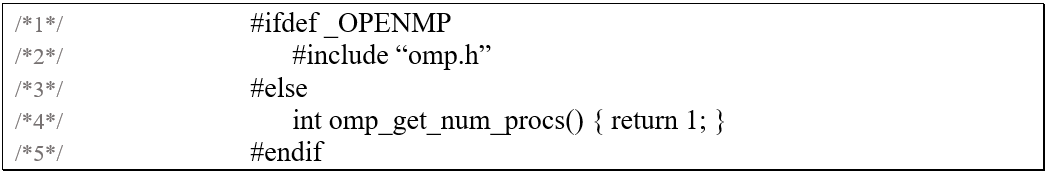
\includegraphics[width=1\textwidth]{lab3Example}
			\end{figure}
		\itemДоказательством того, что программа обладает прямой совместимостью, будет её успешная компиляция без ключа ''–fopenmp'' и корректность расчётов.
		\itemПровести эксперименты, замеряя параллельное ускорения на каждом из пяти этапов, самостоятельно выбрав диапазон значений N и количество экспериментов. Привести графики параллельного ускорения, рассчитанного методом А и методом Б, для каждого этапа и всей программы в целом. 
		\itemНаписать отчёт о проделанной работе с подробными выводами и комментариями полученных результатов (сравнить метод А и метод Б; объяснить влияние параллельного ускорения отдельных этапов на параллельное ускорение всей программы).
	\end{enumerate}
}